\chapter{Paquetes termodinámicos}
	\section{Estructura de la librería}
	 \subsection{Materia Homogénea}

			\begin{figure}[!h]
			  
			  \centering
			    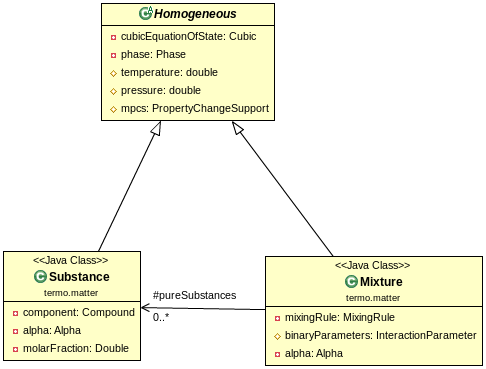
\includegraphics[scale=0.7]{Homogenous.png}
			    \caption{A picture of a gull.}
			\end{figure}

		\subsection{Materia Heterogénea}

			\begin{figure}[!h]
			  
			  \centering
			    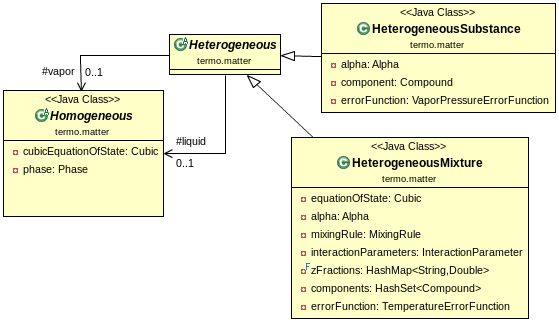
\includegraphics[scale=0.7]{heterogeneous.png}
			    \caption{ads}
			\end{figure}


	
		\subsection{Mezcla}



	\section{Objetos incluidos}
		\subsection{Ecuaciones de estado cúbicas}
		\subsection{Expresiones de $\alpha$}
		\subsection{Reglas de mezclado}
		\subsection{modelos de actividad}
	\section{¿Cómo extender los paquetes?/ ¿Cómo escribir mi propio paquete?}
		\subsection{Fork Repo desde GitHub}
		\subsection{Agregar classes}
		\subsection{Pull Request}
